% ****************************************************************************************
\chapter{Echtzeitversuch}
\label{chap:Echtzeitversuch}
% ****************************************************************************************
Im diesem Kapitel erfolgt die Validierung des in \Chap{Realisierung} beschriebenen Echtzeitsystems. Dazu ist erforderlich, das System auf das in \Chap{Einfuehrung} verlangte Echtzeitkriterium zu untersuchen. Des Weiteren muss nachgewiesen werden, dass die Ergebnisse aus der Simulation in \Sec{sec:Simulation} unter Berücksichtigung der Raumeigenschaften reproduziert werden können.



% ****************************************************************************************
\section{Untersuchung des Zeitverhaltens}
\label{sec:UntersuchungZeitverhalten}
% ****************************************************************************************
Nach dem Echtzeitkriterium aus \Chap{Einfuehrung} müssen alle Rechenoperationen innerhalb der Dauer eines EDMA-Rahmens erfolgt sein. Mit einer Rahmenlänge von 256 (siehe \Sec{subsubsec:WahlSystemparateter}) ergibt das eine Zeit von $T_{EDMA} = 5,33ms$. Die Messung des Zeitverhaltens bei dieser Rahmengröße ergibt, dass das Programm nicht in Echtzeit arbeitet und somit die Dauer des Algorithmus die des EDMA-Blocks überschreitet. Als Lösungsansatz wird zunächst die Möglichkeit untersucht, die Rahmenlänge $L$ zu vergrößern. In Anbetracht der Zweier-Potenz-Regel (siehe \Sec{subsubsec:SchnelleKreuzkorrelatio}) ergibt sich für die nächste Größe eine Anzahl von 512 Abtastwerten und somit eine Zeit von $T_{EDMA} = 10,7ms$. Unter Berücksichtigung der Stationaritätseigenschaft von Sprache (siehe \Sec{subsec:Stationaritaet}) erweist sich diese Dauer als geeignet und wird für den weiteren Verlauf der Arbeit spezifiziert.

\abb{profiling} zeigt das Zeitverhalten des Tracking-Programms bei einer EDMA-Blockgröße von 512 Abtastwerten. Die Zeitmessung des Algorithmus ergibt, dass das Echtzeitkriterium erfüllt wird, da die Summe der einzelnen Funktionszeiten $T_{Algo}$ (siehe \tab{Profiling_Algo}) kleiner ist, als die Dauer eines EDMA-BLocks. 
Werden die Daten jedoch unter Nutzung der UART-Schnittstelle versandt, vergrößert sich die benötigte Zeit und überschreitet die Dauer eines EDMA-Blocks. Da die serielle Schnittstelle für unterschiedliche Übertragungsgeschwindigkeiten (Baudrate) konfiguriert werden kann, wird die Baudrate, wie dargestellt, sukzessiv erhöht. Bei einer Geschwindigkeit von 57600 Baud hat sich die benötigte Zeit zum Senden eines Datenpakets so weit verringert, dass die Dauer eines EDMA-Rahmens insgesamt nicht überschritten wird. Deutlich wird dies auch durch den \code{ADC\_DAC\_LOOP\_THROUGH} (in grün dargestellt). Hierbei wird der Speicherinhalt eines EDMA-Frames innerhalb der Hauptroutine direkt vom ADC-Speicher in den DAC-Speicher kopiert. Kann dieser Vorgang erfolgreich abgeschlossen werden entsteht kein Datenverlust (Sprünge) und der Algorithmus arbeitet in Echtzeit (\abb{Profile_UART_57600}).



\begin{table}[h]
     \center
     \begin{tabular}{lr}
     \hline
          Funktio & Zeit $[\mu s]$\\
           \hline \hline
          \code{ADC\_DAC\_LOOP\_THROUGH}    & 70               \\
          \code{Copy2CmplxStruct}           & 430              \\
          \code{CalcVariance}               & 70               \\
          \code{FastCrossCorrelation}       & 7000     \\
          \code{SearchAndFind}              & 1920     \\
          \code{CreateHistogram}            & 10     \\
          \code{send\_string}               & 940     \\
          \hline
          Summe:                            & 10440\\
          \hline
          \code{EDMA Block}                   & 10600     \\
          \hline
          Reserve:                  & 160     \\
         \hline
     \end{tabular}
  \caption{Profiling des Tracking-Algorithmus}
 \label{tab:Profiling_Algo}
 \end{table}






Zu beachten ist, dass die Echtzeitfähigkeit nur erreicht wird, wenn keine Daten unter Verwendung der seriellen Schnittstelle versandt werden. Grund hierfür sind die zusätzlich benötigten Funktionsaufrufe zum Erstellen des Datenpakets sowie dessen serielle Übertragung.


%\myFigure{real}                  % Figure tag (missing, real)
%         {Big}                 % Size (small,medium,big)
%         {h!}             % z.B. htbp
%         {Untersuchung des Zeitverhaltens der implementierten Methoden}                % Figure title
%         {profiling}                % Figure label 
%         {04_Echtzeitversuch/profiling}     % Path to real figure






% ----------------------------------------- SUB-FIGURE -----------------------------------
\begin{figure}
        \centering
        \begin{subfigure}[b]{0.6\textwidth}
                \centering
                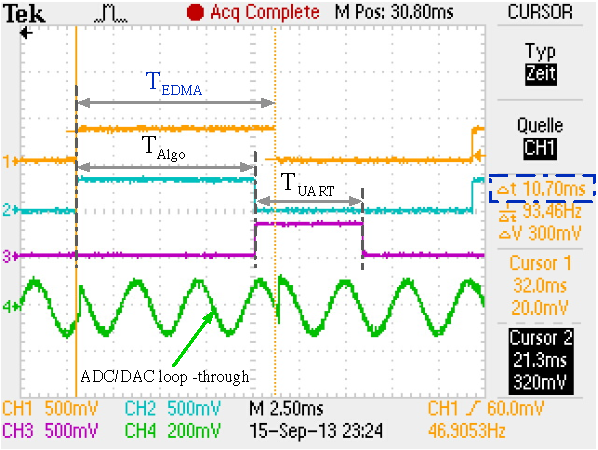
\includegraphics[width=\textwidth]{images/04_Echtzeitversuch/Profile_UART_9600}
                \caption{Baudrate: 9600 Baud}
                \label{fig:Profile_UART_9600}
        \end{subfigure}
        ~ %add desired spacing between images, e. g. ~, \quad, \qquad etc.
          %(or a blank line to force the subfigure onto a new line)
        \begin{subfigure}[b]{0.6\textwidth}
                \centering
                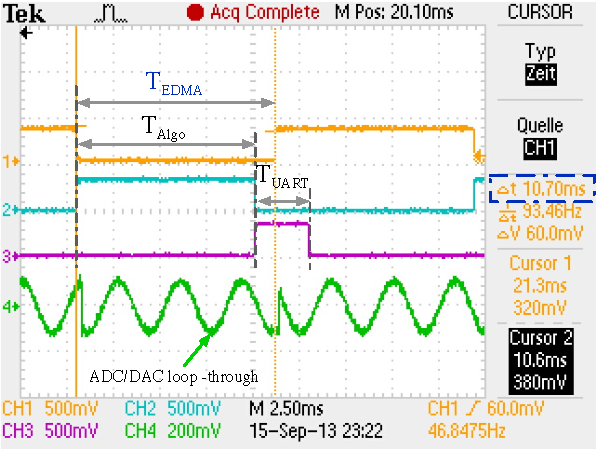
\includegraphics[width=\textwidth]{images/04_Echtzeitversuch/Profile_UART_19200}
                \caption{Baudrate: 19200 Baud}
                \label{fig:Profile_UART_19200}
        \end{subfigure}
        ~ %add desired spacing between images, e. g. ~, \quad, \qquad etc.
          %(or a blank line to force the subfigure onto a new line)
        \begin{subfigure}[b]{0.6\textwidth}
                \centering
                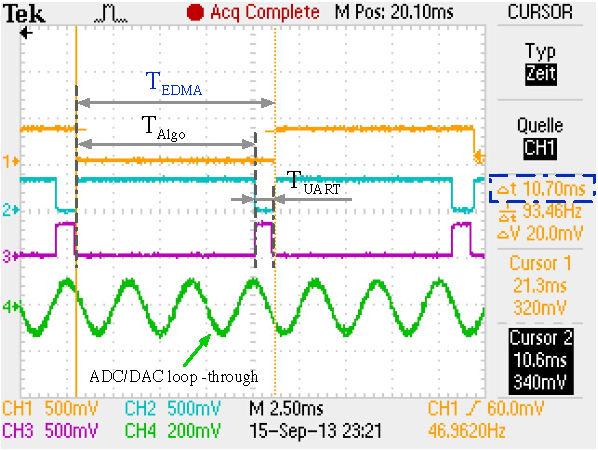
\includegraphics[width=\textwidth]{images/04_Echtzeitversuch/Profile_UART_57600}
                \caption{Baudrate: 57600 Baud}
                \label{fig:Profile_UART_57600}
        \end{subfigure}
        \caption{Untersuchung des Zeitverhaltens mit einer EDMA-Dauer von $T_{EDMA} = 10,7ms$.}
        \label{fig:profiling}
\end{figure}
% ----------------------------------------- SUB-FIGURE -----------------------------------












% ****************************************************************************************
\section{Versuchsaufbau}
\label{sec:Versuchsaufbau}
% ****************************************************************************************
\abb{aufbau_echtzeitmessung} zeigt den schematischen Versuchsaufbau der Echtzeitmessung. Um die Leistung des Systems in akustisch anspruchsvoller Umgebung testen zu können, wurde ein kleiner Raum mit den Abmaßen  $5m \times 3m \times 2,7m$ gewählt. Dieser verfügt über schallharte Wände, so dass die Systemreaktion auf ein diffuses Schallfeld sowie starke Reflexionen untersucht werden können. Zur Einhaltung des in \Sec{subsubsec:Fernfeld} beschriebenen Fernfeldkriteriums bei einer oberen Spracheckfrequenz von 3 kHz wurde ein Abstand von 1,6m gewählt. Zur Einstellung der unterschiedlichen Winkel wird das Array wie in \abb{array_winkeleinteilung} dargestellt drehbar gelagert und erhält ein Winkelaufteilung. Das Array kann so mit Hilfe des \ccs Graph-Windows exakt ausgerichtet werden und anhand der Winkelteilung in genauen Schritten gedreht werden.


\myFigure{real}                  % Figure tag (missing, real)
         {Big}                 % Size (small,medium,big)
         {h!}             % z.B. htbp
         {Versuchsaufbau der Echtzeitmessung}                % Figure title
         {aufbau_echtzeitmessung}                % Figure label 
         {04_Echtzeitversuch/aufbau_echtzeitmessung}     % Path to real figure





\myFigure{real}                  % Figure tag (missing, real)
         {medium}                 % Size (small,medium,big)
         {h!}                     % z.B. htbp
         {Einstellung der theoretischen Winkel am Mikrofonarray}                % Figure title
         {array_winkeleinteilung}                % Figure label 
         {04_Echtzeitversuch/array_winkeleinteilung}     % Path to real figure



% ****************************************************************************************
\section{Ergebnisse}
\label{sec:Ergebnisse}
% ****************************************************************************************
Im Folgenden wird zunächst ein grundlegender Funktionstest des Algorithmus durchgeführt. Anschließend erfolgt eine Verifikation der Winkelauflösung. Auf Grund der hohen Anzahl von Raumwinkelkombinationen werden im Rahmen dieses Tests nur einige ausgewählt, so dass eine Tendenz sichtbar werden kann.




% ****************************************************************************************
\subsection{Funktionstest}
\label{subsec:Funktionstest}
% ****************************************************************************************
Zum grundlegenden Test der Algorithmusfunktionalität wurden, wie in \abb{test_echtzeit_grundfunktion} dargestellt, vier verschiedene Schalleinfallsrichtungen eingestellt. Als Quellsignal diente eine Testdatei mit männlicher Sprache. Die Einstellungen der Histogrammglättung wurden mit einer Ringspeicherlänge von 20 und einer Schwelle von 20\% vorgenommen.

Es ist zunächst zu erkennen, dass der Algorithmus die Raumwinkel sicher detektiert. Auf Grund der endlich genauen Möglichkeit das Array zum Lautsprecher auszurichten, kann davon ausgegangen werden, dass Winkelfehler von einem Auflösungsschritt auf diese Einstellungstoleranz zurückzuführen sind. Die darüber hinaus auftretenden starken Winkelsprünge können den durch die Raumwände verursachten Reflexionen zugeschrieben werden. 
          


% ----------------------------------------- SUB-FIGURE -----------------------------------
\begin{figure}
        \centering
        \begin{subfigure}[b]{0.48\textwidth}
                \centering
                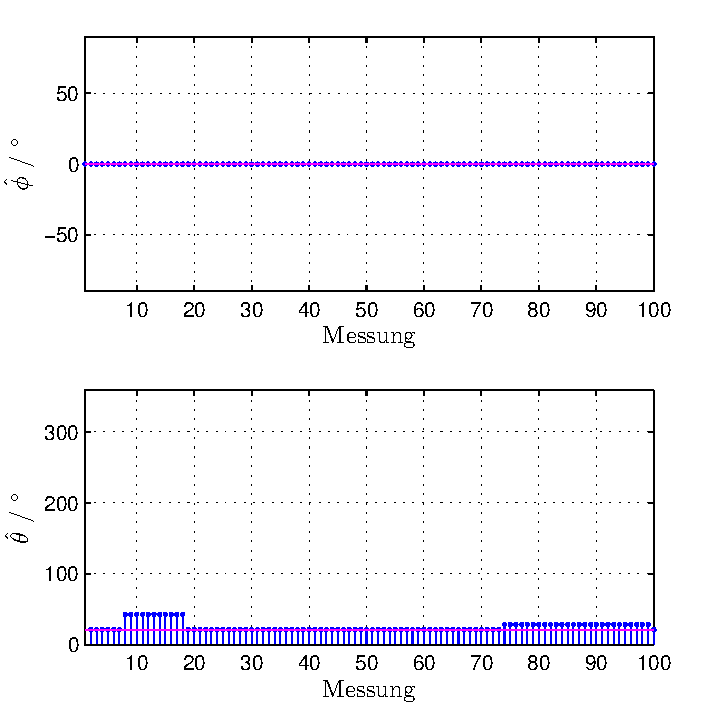
\includegraphics[width=\textwidth]{images/04_Echtzeitversuch/MALE_Phi_0_Theta_21}
                \label{fig:Foto_DSP_Draufsicht_Seitanansicht}
                \caption{$\phi=0°, \theta = 21°$}
        \end{subfigure}
        ~ %add desired spacing between images, e. g. ~, \quad, \qquad etc.
          %(or a blank line to force the subfigure onto a new line)
        \begin{subfigure}[b]{0.48\textwidth}
                \centering
                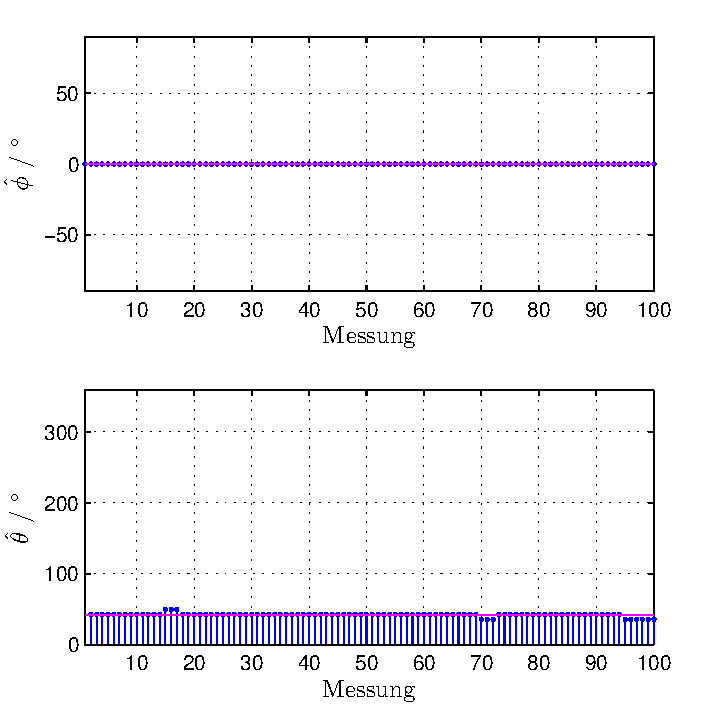
\includegraphics[width=\textwidth]{images/04_Echtzeitversuch/MALE_Phi_0_Theta_42}
                \label{fig:Foto_DSP_Draufsicht}
                \caption{$\phi=0°, \theta = 42°$}
        \end{subfigure}
        ~ %add desired spacing between images, e. g. ~, \quad, \qquad etc.
          %(or a blank line to force the subfigure onto a new line)
        \begin{subfigure}[b]{0.48\textwidth}
                \centering
                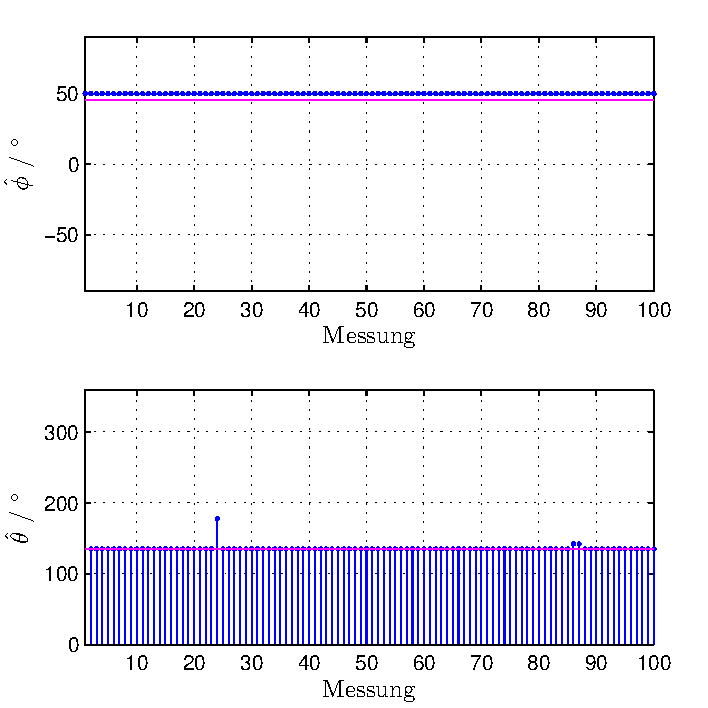
\includegraphics[width=\textwidth]{images/04_Echtzeitversuch/MALE_Phi_45_Theta_135}
                \label{fig:Foto_DSP_Draufsicht}
                \caption{$\phi=45°, \theta = 135°$}
        \end{subfigure}
        ~ %add desired spacing between images, e. g. ~, \quad, \qquad etc.
          %(or a blank line to force the subfigure onto a new line)
        \begin{subfigure}[b]{0.48\textwidth}
                \centering
                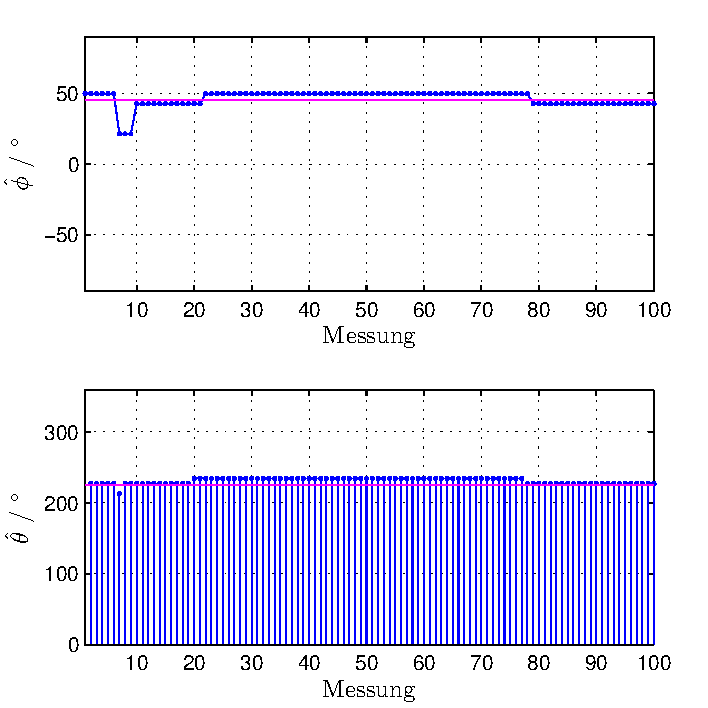
\includegraphics[width=\textwidth]{images/04_Echtzeitversuch/MALE_Phi_45_Theta_225}
                \label{fig:Foto_DSP_Draufsicht}
                \caption{$\phi=45°, \theta = 225°$}
        \end{subfigure}
        \stepcounter{missingFigureCount}
        \caption{Messung der Schalleinfallsrichtung aus unterschiedlichen Winkeln in einem hallenden Raum.}
        \label{fig:test_echtzeit_grundfunktion}
\end{figure}
% ----------------------------------------- SUB-FIGURE -----------------------------------



% ****************************************************************************************
\subsection{Verifikation der Winkelauflösung}
\label{subsec:VerifikationWinkelaufloesung}
% ****************************************************************************************
Zur Verifikation der Winkelauflösung wird das Mikrofonarray zunächst auf $\phi=0°$ und $\theta=0°$ ausgerichtet. Anschließend erfolgt eine Rotation um $\theta$ in Abständen der Winkelauflösung. Der Winkel $\theta$ wird dabei die Werte $0° \leq \theta \leq 92°$ annnehmen.
 
\abb{verifikation_winkelaufloesung_1} und \abb{verifikation_winkelaufloesung_2} illustrieren die Messergebnisse bei einer Anzahl von 100 Messungen pro Winkel. Hier wird ersichtlich, dass die Winkel im Abstand der in  \Sec{subsubsec:Winkelaufloesung} beschriebenen Winkelauflösung eingenommen werden können. Die Abweichungen um einen Winkelschritt sind erneut auf die begrenzte Einstellgenauigkeit zurückzuführen. Auf Grund von Reflexion ergeben sich hier erneut vereinzelte Fehler in Form von abrupten Winkelsprüngen.


% ----------------------------------------- SUB-FIGURE -----------------------------------
\begin{figure}
        \centering
        \begin{subfigure}[b]{0.48\textwidth}
                \centering
                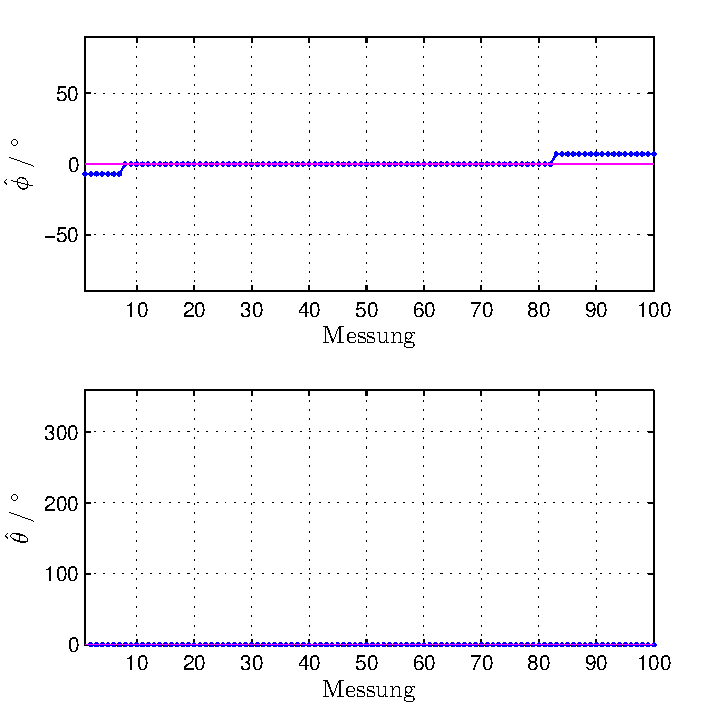
\includegraphics[width=\textwidth]{images/04_Echtzeitversuch/MALE_Phi_0_Theta_0}
                \label{fig:Foto_DSP_Draufsicht_Seitanansicht}
                \caption{$\phi=0°, \theta = 0°$}
        \end{subfigure}
        ~ %add desired spacing between images, e. g. ~, \quad, \qquad etc.
          %(or a blank line to force the subfigure onto a new line)
        \begin{subfigure}[b]{0.48\textwidth}
                \centering
                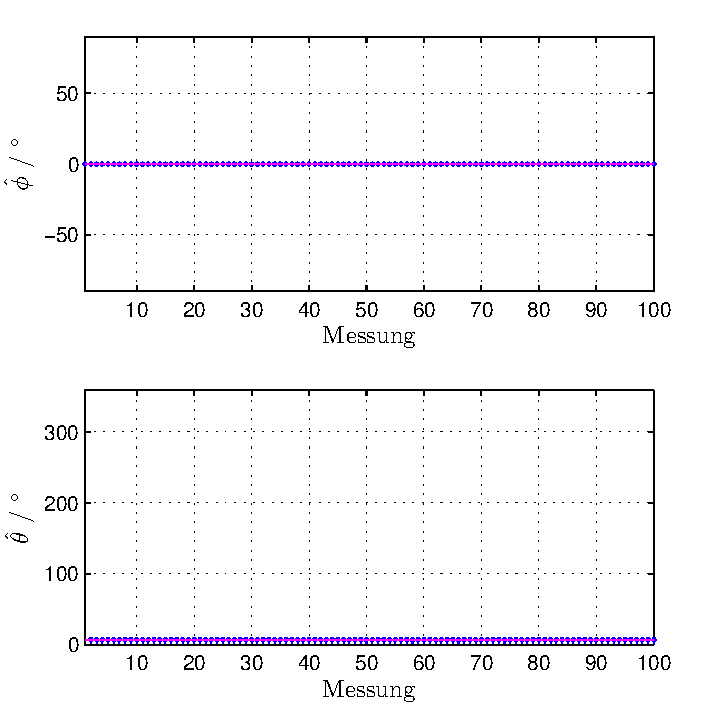
\includegraphics[width=\textwidth]{images/04_Echtzeitversuch/MALE_Phi_0_Theta_7}
                \label{fig:Foto_DSP_Draufsicht}
                \caption{$\phi=0°, \theta = 7°$}
        \end{subfigure}
        ~ %add desired spacing between images, e. g. ~, \quad, \qquad etc.
          %(or a blank line to force the subfigure onto a new line)
        \begin{subfigure}[b]{0.48\textwidth}
                \centering
                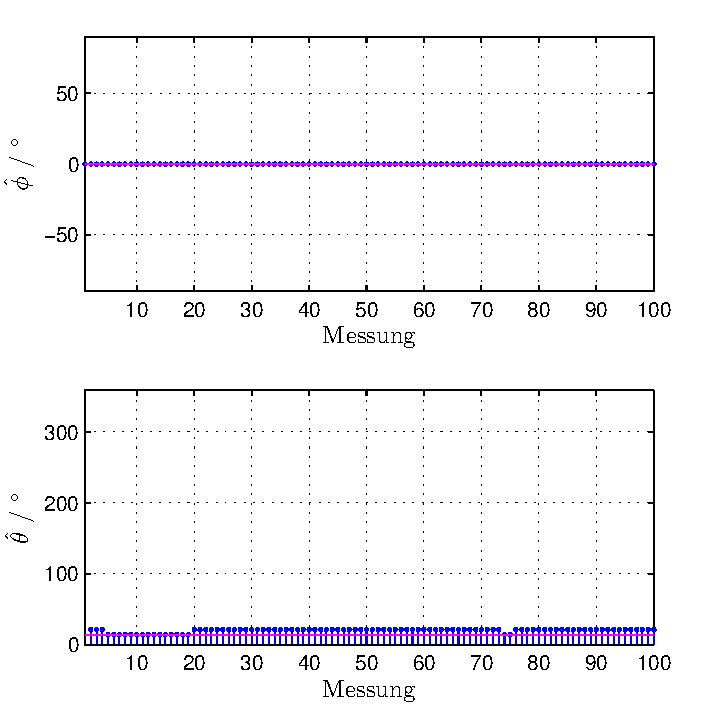
\includegraphics[width=\textwidth]{images/04_Echtzeitversuch/MALE_Phi_0_Theta_14}
                \label{fig:Foto_DSP_Draufsicht}
                \caption{$\phi=0°, \theta = 14°$}
        \end{subfigure}
        ~ %add desired spacing between images, e. g. ~, \quad, \qquad etc.
          %(or a blank line to force the subfigure onto a new line)
        \begin{subfigure}[b]{0.48\textwidth}
                \centering
                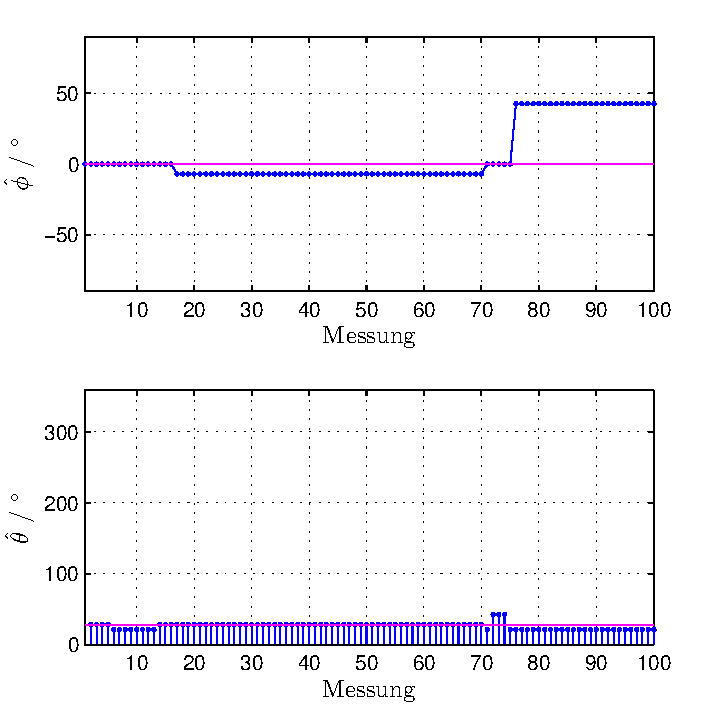
\includegraphics[width=\textwidth]{images/04_Echtzeitversuch/MALE_Phi_0_Theta_28}
                \label{fig:Foto_DSP_Draufsicht}
                \caption{$\phi=0°, \theta = 28°$}
        \end{subfigure}
         ~ %add desired spacing between images, e. g. ~, \quad, \qquad etc.
          %(or a blank line to force the subfigure onto a new line)
        \begin{subfigure}[b]{0.48\textwidth}
                \centering
                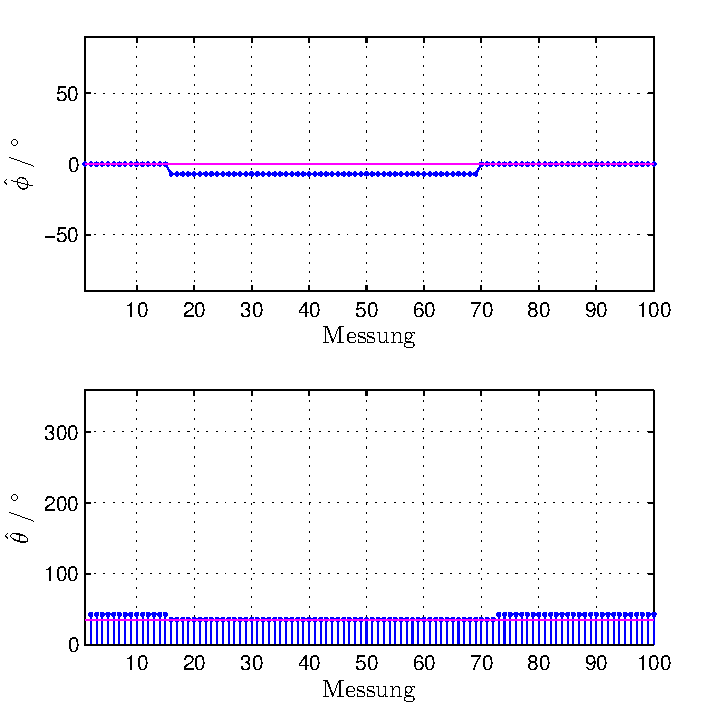
\includegraphics[width=\textwidth]{images/04_Echtzeitversuch/MALE_Phi_0_Theta_35}
                \label{fig:Foto_DSP_Draufsicht}
                \caption{$\phi=0°, \theta = 35°$}
        \end{subfigure}
        ~ %add desired spacing between images, e. g. ~, \quad, \qquad etc.
          %(or a blank line to force the subfigure onto a new line)
        \begin{subfigure}[b]{0.48\textwidth}
                \centering
                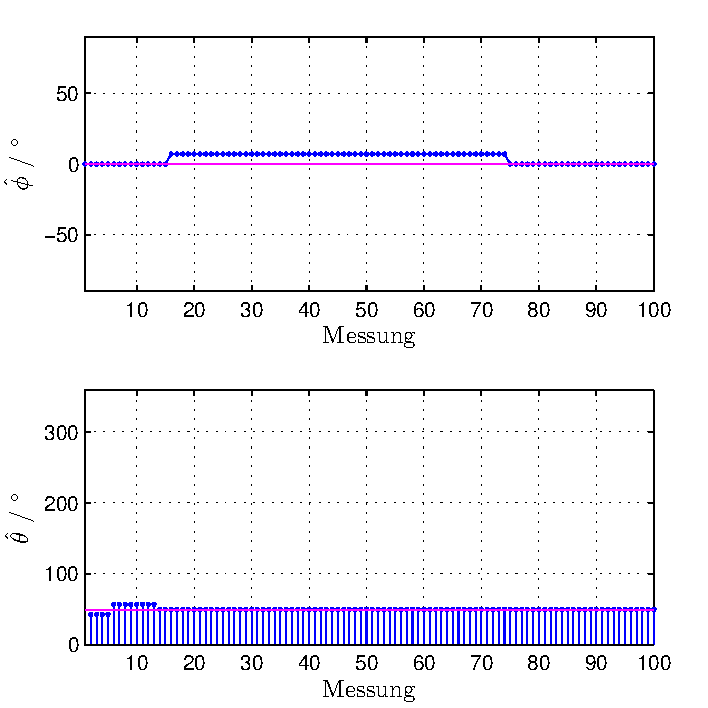
\includegraphics[width=\textwidth]{images/04_Echtzeitversuch/MALE_Phi_0_Theta_49}
                \label{fig:Foto_DSP_Draufsicht}
                \caption{$\phi=0°, \theta = 49°$}
        \end{subfigure}
        \stepcounter{missingFigureCount}
        \caption{Verifikation der Winkelauflösung im Bereich $0° \leq \theta \leq 49°$.}
        \label{fig:verifikation_winkelaufloesung_1}
\end{figure}
% ----------------------------------------- SUB-FIGURE -----------------------------------









% ----------------------------------------- SUB-FIGURE -----------------------------------
\begin{figure}
        \centering
        \begin{subfigure}[b]{0.48\textwidth}
                \centering
                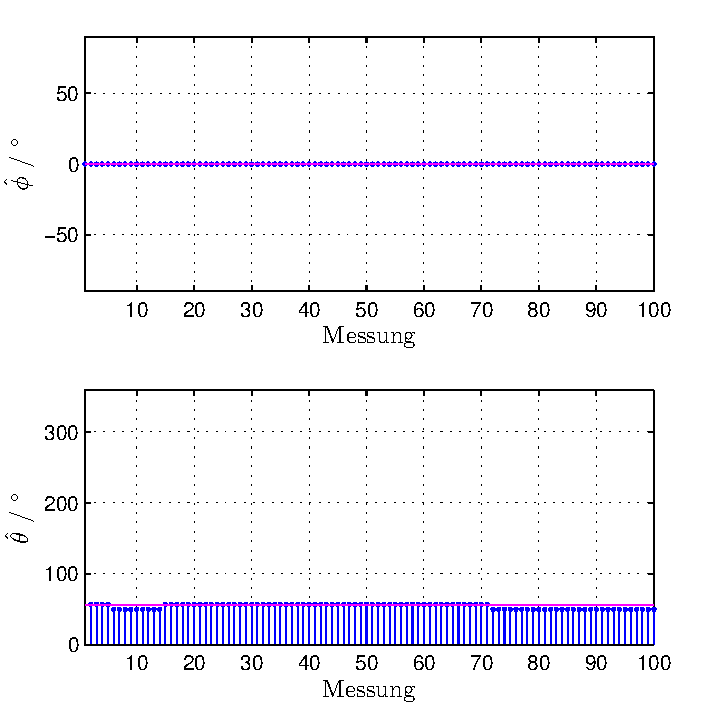
\includegraphics[width=\textwidth]{images/04_Echtzeitversuch/MALE_Phi_0_Theta_56}
                \label{fig:Foto_DSP_Draufsicht_Seitanansicht}
                \caption{$\phi=0°, \theta = 56°$}
        \end{subfigure}
        ~ %add desired spacing between images, e. g. ~, \quad, \qquad etc.
          %(or a blank line to force the subfigure onto a new line)
        \begin{subfigure}[b]{0.48\textwidth}
                \centering
                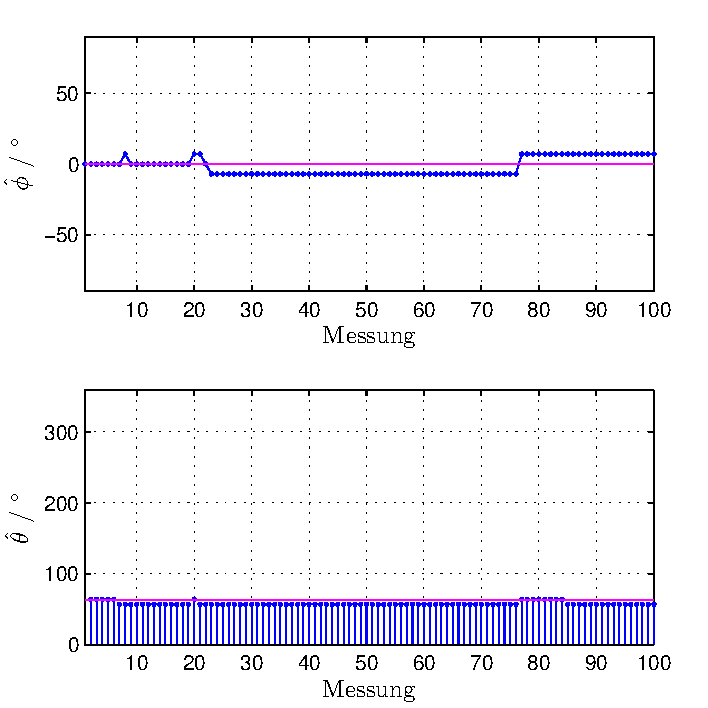
\includegraphics[width=\textwidth]{images/04_Echtzeitversuch/MALE_Phi_0_Theta_63}
                \label{fig:Foto_DSP_Draufsicht}
                \caption{$\phi=0°, \theta = 63°$}
        \end{subfigure}
        ~ %add desired spacing between images, e. g. ~, \quad, \qquad etc.
          %(or a blank line to force the subfigure onto a new line)
        \begin{subfigure}[b]{0.48\textwidth}
                \centering
                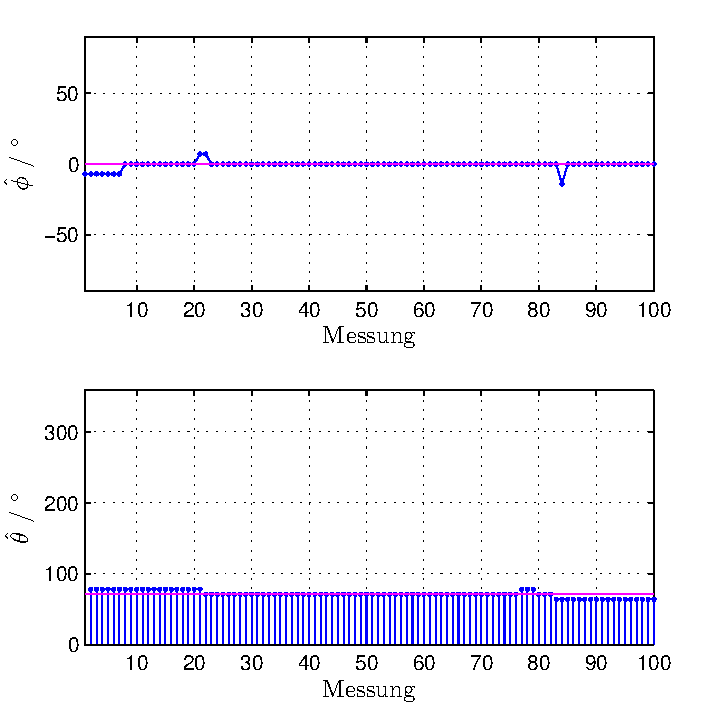
\includegraphics[width=\textwidth]{images/04_Echtzeitversuch/MALE_Phi_0_Theta_71}
                \label{fig:Foto_DSP_Draufsicht}
                \caption{$\phi=0°, \theta = 71°$}
        \end{subfigure}
        ~ %add desired spacing between images, e. g. ~, \quad, \qquad etc.
          %(or a blank line to force the subfigure onto a new line)
        \begin{subfigure}[b]{0.48\textwidth}
                \centering
                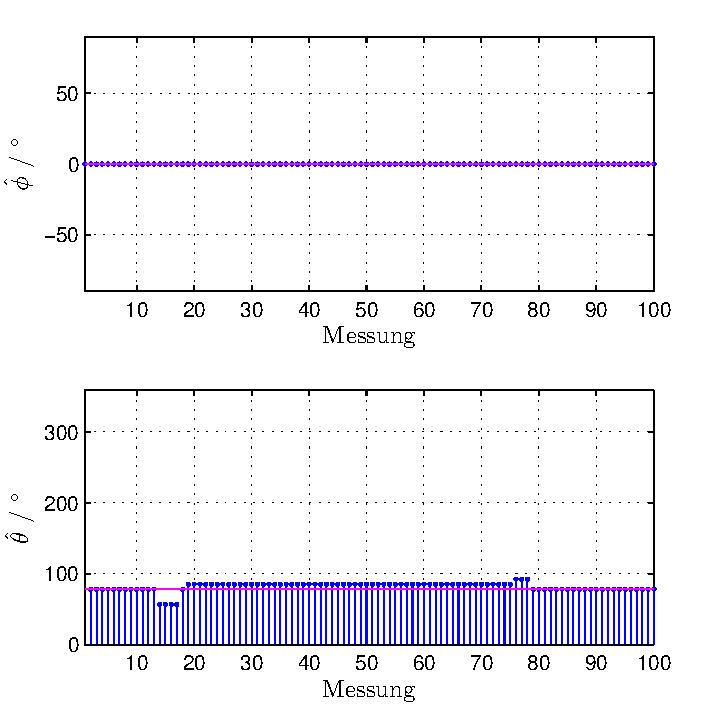
\includegraphics[width=\textwidth]{images/04_Echtzeitversuch/MALE_Phi_0_Theta_78}
                \label{fig:Foto_DSP_Draufsicht}
                \caption{$\phi=0°, \theta = 78°$}
        \end{subfigure}
         ~ %add desired spacing between images, e. g. ~, \quad, \qquad etc.
          %(or a blank line to force the subfigure onto a new line)
        \begin{subfigure}[b]{0.48\textwidth}
                \centering
                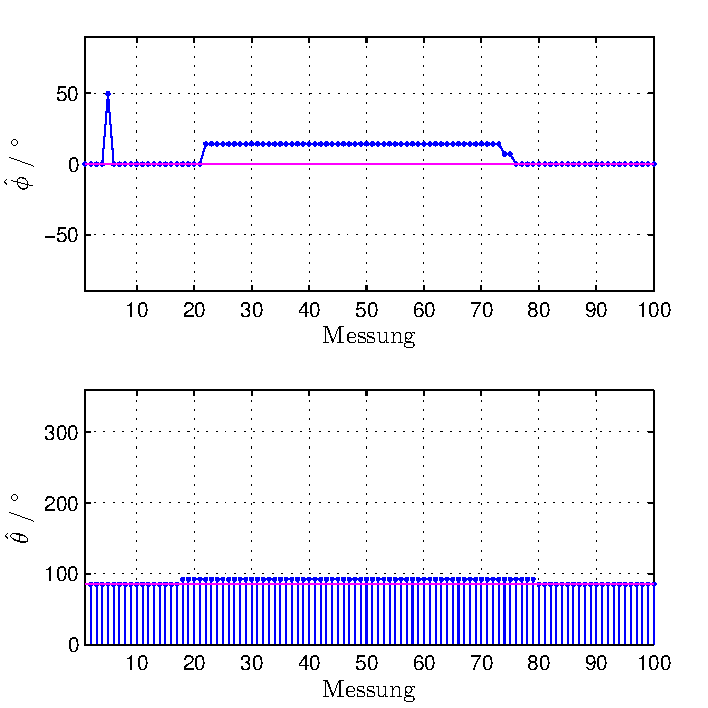
\includegraphics[width=\textwidth]{images/04_Echtzeitversuch/MALE_Phi_0_Theta_85}
                \label{fig:Foto_DSP_Draufsicht}
                \caption{$\phi=0°, \theta = 85°$}
        \end{subfigure}
        ~ %add desired spacing between images, e. g. ~, \quad, \qquad etc.
          %(or a blank line to force the subfigure onto a new line)
        \begin{subfigure}[b]{0.48\textwidth}
                \centering
                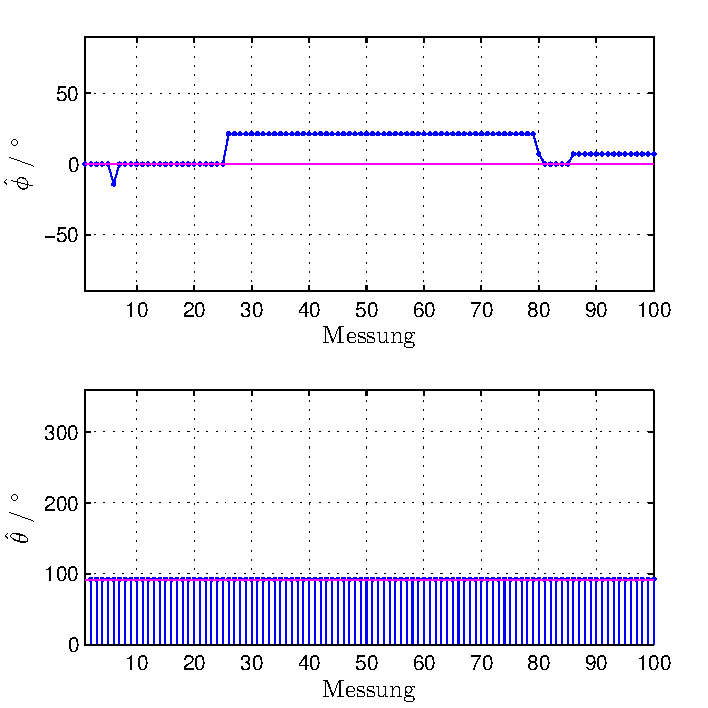
\includegraphics[width=\textwidth]{images/04_Echtzeitversuch/MALE_Phi_0_Theta_92}
                \label{fig:Foto_DSP_Draufsicht}
                \caption{$\phi=0°, \theta = 92°$}
        \end{subfigure}
        \stepcounter{missingFigureCount}
        \caption{Verifikation der Winkelauflösung im Bereich $56° \leq \theta \leq 92°$.}
        \label{fig:verifikation_winkelaufloesung_2}
\end{figure}
% ----------------------------------------- SUB-FIGURE -----------------------------------


